% TeX source
%
% Author: Tetsuya Ishikawa <tiskw111@gmail.com>
% Date  : March 20, 2020
%%%%%%%%%%%%%%%%%%%%%%%%%%%%%%%%%%%% SOURCE START %%%%%%%%%%%%%%%%%%%%%%%%%%%%%%%%%%%

\subsection{カーネルサポートベクターマシンとカーネル回帰}

線形SVMでは,回帰曲面を超平面$y = \bs{w}\tran\bs{x}$としたが,
回帰曲線を一般の$f_w(\bs{x})$とした場合,SVMは次のように一般化される.
\begin{align}
    \label{eqn:general_svm_1}
    y &= \Sgn \left( f_w(\bs{x}) \right), \\
    \label{eqn:general_svm_2}
    w &= \argmin_{w} \sum_{i \in \mathcal{I}} V_{\mathrm{svm}}
    \left( y_i - f_w(\bs{x}_i) \right),
\end{align}
ただし$w$は回帰曲線のパラメータである.
先に見た通り,式(\ref{eqn:general_svm_2})の最適化問題は
\begin{equation}\begin{split}
    \label{eqn:general_svm_3}
    \min_{\xi_i, i \in \mathcal{I}} \hspace{6pt}& \sum_{i \in \mathcal{I}} \xi_i, \\
    \text{s.t.} \hspace{6pt}
    & \xi_i \geq 1 - y_i f_w(\bs{x}_i), \hspace{ 5pt} \text{for all $i \in \mathcal{I}$}, \\
    & \xi_i \geq 0,                     \hspace{55pt} \text{for all $i \in \mathcal{I}$},
\end{split}\end{equation}
と等価である.
回帰曲線$f_w$としてどのような曲線を用いるかによってSVMの柔軟性が大きく左右されるのだが,
回帰曲線として無限大の自由度を持つカーネル回帰を採用したのがK-SVMである.
カーネル回帰 (\textit{kernel regression}) とは,適切に選ばれた関数の無数の足し合わせで回帰曲線を構成する手法であり,
先に述べたとおり,無限の自由度を有する回帰手法である.本小節では,まずはこのカーネル回帰について見てみよう.

\begin{note}
「適切」とは,カーネル関数が対称かつ正定値になるように,という意味である.
しかし本節ではそこまでは踏み込まないため,
「厳密に任意ではないが,とりあえずガウス関数ならオッケー」程度に考えて頂ければ十分である.
\end{note}

簡単のため,$x$も$f_w(x)$も1次元の実数変数であるとしよう.このとき,カーネル回帰は回帰曲線を
\begin{equation}
\label{eqn:kernel_reg}
f_w(x) \triangleq \int_{-\infty}^{\infty} w(p) \phi(x, p) \, \mathrm{d}p,
\end{equation}
とおく手法である.
ただし$f_w$は回帰曲線,$\phi$は任意に定められた関数,$w$はパラメータ関数であり,$\phi$は事前に与えておく関数,
パラメータ関数$w$は与えられたデータ点群に最もよくフィットするものを最適化によって求めるものとする.
関数$\phi$はどのように与えても良いが,頻繁に用いられる$\phi$の例として,標準偏差$\sigma$の正規分布
\begin{equation}
G_\sigma(x) \triangleq \frac{1}{\sqrt{2\pi}\sigma}
\exp \left( -\frac{x^2}{2\sigma^2} \right),
\end{equation}
を$x$方向に$p$だけ平行移動した関数が挙げられる.すなわち
\begin{equation}
\phi(x, p)
= G_\sigma (x - p)
= \frac{1}{\sqrt{2\pi}\sigma} \exp \left( -\frac{(x - p)^2}{2\sigma^2} \right),
\end{equation}
である.このとき$f_w$は
\begin{equation}
f_w(x) = \int_{-\infty}^{\infty} w(p) G_\sigma (x - p) \, \mathrm{d}p,
\end{equation}
となる.上式を見れば分かるように,正規分布を平行移動しつつ,
重み$w$をかけながら足し込むというやり方で回帰曲線を構成している.
この回帰は,後に説明するように,RBFカーネル (\textit{radial basis function}) と呼ばれるものに相当する.
以下では一般の$\phi$に対して議論を進めていくが,具体性の欲しい読者は$\phi(x, p) = G_\sigma(x - p)$として読み進めて構わない.

さて,回帰曲線の関数系が定まったところで,次は回帰曲線のパラメータ関数$w$の決定の仕方について説明しよう.
パラメータ関数$w$の決定の仕方は様々な方法があるが,ここでは最も簡単な最小2乗法を紹介する.
回帰のデータ点群を
\begin{equation}
\mathcal{D} \triangleq \bigl\{
(x_i, y_i) \bigm| x_i \in \mathbb{R}, \, y_i \in \mathbb{R}, \, i \in
\mathcal{I} \bigr\},
\end{equation}
とすると,パラメータ関数$w$は最適化問題
\begin{equation}
\label{eqn:kernel_reg_w_naive}
\min_{w} \sum_{i \in \mathcal{I}}
\bigl( y_i - f_w(x_i) \bigr)^2
\end{equation}
を解くことで求めることが出来そうな気がするが,実は式(\ref{eqn:kernel_reg_w_naive})はあまり好ましくない.
注意すべき点として,式(\ref{eqn:kernel_reg})で定められる回帰曲線$f_w$のパラメータは関数$w$であるから,
曲線$f_w$は「関数1つ分」の自由度を持つ.これは実数に換算すると「無限個分」の自由度である.
回帰に与えられるデータ点群は高々有限個しかないため,曲線$f_w$はそれらのデータ点をすべて通ることができてしまい,
さらにそのようなパラメータ関数$w$は無数に存在する.これは次の2つの理由で好ましくない.
1つ目の理由は,単純に式(\ref{eqn:kernel_reg_w_naive})が唯一解を持たない点である.
唯一解を持たない最適化問題は,数学的に解きにくいだけでなく,応用上は最適解として得られた関数のうちどれが良いかを
さらに選択しなければいけないという意味で,あまり便利とは言えない.
そして2つ目の理由は,こちらの方がより重要なのであるが,汎化性能に欠ける曲線が出来上がってしまう点である.
一般に回帰問題でよく言われるように,与えられたデータ点をすべて通る回帰曲線は好ましくない.
回帰の目的の1つに予測がある.すなわち回帰で得られた曲線を予測に使用するケースが機械学習ではよくあるが,
与えられたデータ点をすべて通ってしまうような曲線は,凹凸が激しく荒れた曲線になりやすいため,
予測という観点からは役に立たないことが多い.この現象は過学習 (\textit{over fitting}) と呼ばれており,
与えられたデータ点に対して回帰曲線の自由度が高すぎる場合に発生することが知られている.
通常の回帰問題,例えば線形回帰であれば,データ量が少ないからデータ点を増やす,
あるいは回帰曲線自由度が高すぎるからモデル式の次数を下げるなどの対策が取られる.
しかしカーネル回帰の場合,そもそもの自由度が無限大であるから,
いくらデータ点を増やしても足りることはないし,モデル式の自由度を下げることも出来ない.
そこでカーネル回帰では,式(\ref{eqn:kernel_reg_w_naive})に正則化項,すなわち
パラメータ関数$w$が無駄に大きくならないように抑える効果を持つ項を付け加えた形
\begin{equation}
\label{eqn:kernel_reg_w}
\min_{w} \sum_{i \in \mathcal{I}} \bigl( y_i - f_w(x_i) \bigr)^2
+ \lambda \int_{-\infty}^{\infty} |w(p)|^2 \, \mathrm{d}p,
\end{equation}
に修正することで,過学習の問題を解決している.ただし$\lambda$は正の実数パラメータである.
これでめでたく無限の自由度を持つ回帰を実現することが出来るのだが,
読者はまだ上式の第2項が正則化項に見えていないであろう.
これを説明するためには関数解析に関する多少の知識が必要である.
そこで,少しだけ関数解析の世界に寄り道をして,カーネル回帰に必要な知識をご説明しよう.

\begin{figure}[t]
\centerline{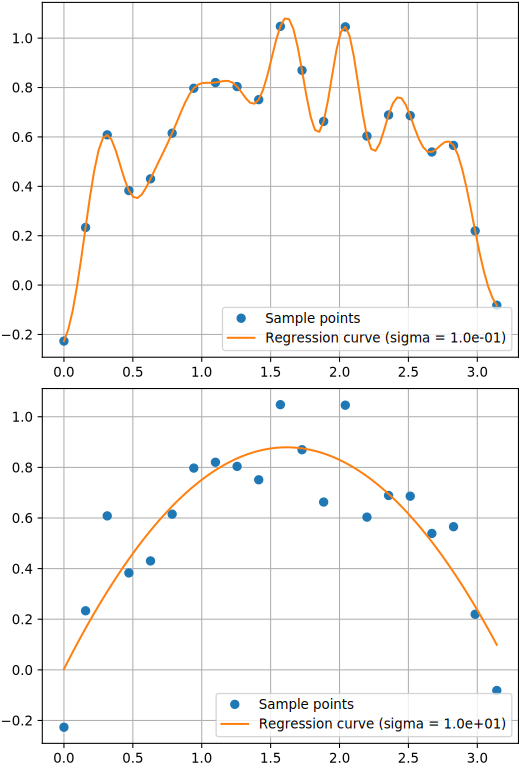
\includegraphics[clip,width=230pt]{figures/overfitting.pdf}}
\caption{回帰問題において過学習した例(上)と過学習を避けることのできた例(下)}
\label{fig:overfitting}
\end{figure}


\subsection{関数空間の導入}

座標平面$\mathbb{R}^2$や座標空間$\mathbb{R}^3$,
一般に実$n$次元空間$\mathbb{R}^n$は,実に便利な数学的解析ツールである.
機械設計をするときも,データ解析をするときも,経済学をするときでさえ,
我々は実$n$次元空間上で数理的な解析をすることが多い.
なぜ実$n$次元空間は便利なのだろうか.
理由は色々と考えられるであろうが,成分表示が出来るからでは決してあるまい.
ベクトルを$\bs{x}$などの一つの記号で置くことで実数の組であることを忘れ,
和や定数倍,ノルム(絶対値),内積,外積などの各種ツールや概念を駆使することで
解析をすることの価値を,我々はすでに知っている.
先人らはその価値を,実数の組であるベクトル以外にも適用しようとした.
すなわち,実数の組でない要素,例えば関数に対し,
和や定数倍,ノルム,内積などを定義することで,
関数をより扱いやすいものにしようと試みた.
その成果が現在のHilbert空間である.
本文書では,Hilbert空間のひとつであり,
関数解析の入り口でもある$L^2$空間について紹介する.

関数$f : \mathbb{R} \to \mathbb{R}$に関する次の積分
\begin{equation}
\int_{-\infty}^{\infty} |f(x)|^2 \, \mathrm{d}x,
\end{equation}
が有限確定の値を持つとき,関数$f$は2乗可積分であると言われる.
2乗可積分な関数の集合を$L^2$空間と定義しよう.すなわち
\begin{equation}
L^2 \triangleq
\left\{ f : \mathbb{R} \to \mathbb{R} \biggm| \int_{-\infty}^{\infty} |f(x)|^2 \, \mathrm{d}x < \infty \right\},
\end{equation}
である.
積分区間はどのようにとっても構わないが,一度定めたらそれを一貫して使い続けなければならないことに注意せよ.
ここではK-SVMへの応用を見越して積分区間は$(-\infty, \infty)$としている.
さて,これから$L^2$空間の要素である関数に対し,和,定数倍,ノルム,内積を定義するのだが,
和と定数倍は通常の関数の和と定数倍でよいので割愛する.関数$f$, $g \in L^2$に対し,
$f$と$g$の内積$\langle f, g \rangle$を
\begin{equation}
\langle f, g \rangle \triangleq \int_{-\infty}^{\infty} f(x) g(x) \, \mathrm{d}x,
\end{equation}
と定義する.実ベクトル空間の場合と同じく,内積$\langle f, g \rangle$は実数値である.
内積$\langle f, g \rangle$が0のとき,関数$f$, $g$は直交すると言われる.
関数$f \in L^2$のノルム$\| f \|$を,$f$同士の内積の平方根として定義する.すなわち
\begin{equation}
\| f \| \triangleq \sqrt{\langle f, f \rangle}
= \sqrt{\int_{-\infty}^{\infty} |f(x)|^2 \, \mathrm{d}x},
\end{equation}
である.
$L^2$空間の定義より,任意の関数$f$, $g \in L^2$に対して,
$\langle f, g \rangle$および$\| f \|$が有限確定の値を持つことが直ちに証明できる.
つまり$f, g \in L^2$であれば$\langle f, g \rangle$や$\| f \|$を安心して使うことができる,
ということだ.

さて,内積やノルムの性質をいくつか確認しておこう.
まずは内積の性質を,定理という形でまとめておく.

\begin{theorem}[関数空間$L^2$上の内積の性質]
以下,$f, g, h \in L^2$, $a, b \in \mathbb{R}$とする.
関数空間$L^2$上の内積$\langle \cdot, \cdot \rangle$について次が成り立つ:
\begin{itemize}
    \item 可換性:$\langle f, g \rangle = \langle g, f \rangle$
    \item 双線形性:$\langle a f + b g, h \rangle = a \langle f, h \rangle + b \langle g, h \rangle$
    \item シュワルツの不等式: $\langle f, g \rangle = \| f \| \, \| g \|$
\end{itemize}
\end{theorem}
\begin{proof}
可換性,双線形性はいずれも内積の定義より自明であるため割愛する.
シュワルツの不等式(\textit{Schwarz inequality})は本文書には直接は関係がないため,
証明は末尾の付録で行う.
\end{proof}

次はノルムの性質を,こちらも定理という形でまとめておく.

\begin{theorem}[関数空間$L^2$上のノルムの性質]
以下,$f, g, h \in L^2$とする.
関数空間$L^2$上のノルム$\| \cdot \|$について次が成り立つ:
\begin{itemize}
    \item 正値性:$\| f \| \geq 0$
    \item 正定性:$\| f \| = 0 \, \Longleftrightarrow \, f = \underline{0}$
    \item 三角不等式:$\| f + g \| \leq \| f \| + \| h \|$
\end{itemize}
\end{theorem}
\begin{proof}
正値性はノルムの定義から自明,正定性も定義よりほぼ自明であろう.
三角不等式は本文書には直接関係しないため,証明は末尾の付録で行う.
\end{proof}

\begin{note}
正定性って本当に自明か?と疑問に思った読者は良い直感をお持ちである.
お気付きの通り,零関数とは異なるが積分すれば0になる関数などいくらでも存在する.
例えばディリクレ関数(\textit{Dirichlet function})が良い例である.
これは,著者が関数空間$L^2$における等号$=$を真面目に定義せずに先に進んでしまったことが
原因なのだが,これは本文書の範囲内を越える.何でもかんでもひとつの文書に詰め込むのは著者の好みではない.
したがって,この点は興味ある読者への愛ある課題として残しておく.
詳細は成書を参照されたい.
\end{note}

関数空間が実ベクトル空間と感覚的にはほぼ同じであるということを体感してもらうために,
例題を1つ紹介する.

\noindent\textsf{例題}\\
実数$a$をパラメータとする積分値
\begin{equation}
I(a) = \int_{-\infty}^{\infty} \bigl| f(x) + a g(x) \bigr|^2 \, \mathrm{d}x,
\end{equation}
を最小化するパラメータ$a = a^*$を求めよ.
ただし関数$f$, $g \in L^2$とし,$g$は零関数ではないとする.

\noindent\textsf{解1}:直接計算による.
\begin{align*}
I(a) &= \| f + a g \|^2 = \| f \|^2 + 2 a \langle f, g \rangle + a^2 \| g \|^2, \\
\therefore \hspace{5pt} a^* &= - \frac{\langle f, g \rangle}{\| g \|^2}
\end{align*}
\hfill$\blacksquare$

\noindent\textsf{解2}:定義より$I(a) = \| f + a g \|^2$であるから,
$I(a)$は関数空間上の直線$f + a g$と原点との距離の2乗である.
よって,図\ref{fig:functional_example_sol2}より,
この距離が最小になるのは,$f + a g$と$g$が直交するときである.したがって
\begin{align*}
\langle f + a^* g, g \rangle &= 0, \\
\langle f, g \rangle + a \| g \|^2 &= 0, \\
\therefore \hspace{5pt} a^* &= - \frac{\langle f, g \rangle}{\| g \|^2}
\end{align*}
\hfill$\blacksquare$

\begin{figure}[t]
\centerline{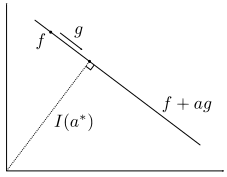
\includegraphics[clip,width=120pt]{figures/functional_example_sol2.pdf}}
\caption{関数空間をベクトル空間のように表現したイメージ図}
\label{fig:functional_example_sol2}
\end{figure}

これ以外にも,線形代数で学んだ定理や性質が,関数空間$L^2$についてもほとんど成り立つ.
大学の線形代数の授業では,実ベクトルであるということを使わずにあえて抽象的な議論で
定理や性質の証明を進めていたであろう.そのため,実ベクトルであれば
成立するのはあたりまえジャン!とか思うような定理に対しても,逐一証明を与えていたはずである.
これは,実ベクトル以外の対象を想定してのことであり,まさに今,その状況に出会ったという訳である.


\subsection{カーネル回帰の定式化}

さて,話をカーネル回帰に戻そう.
カーネル回帰の回帰曲線$f_w$は式(\ref{eqn:kernel_reg})で定義されるが,
関数$\phi(x, p)$を分かり易さのために$\phi_x(p)$と書き表すことにすれば,
\begin{equation}
f_w(x) = \langle w, \phi_x \rangle,
\end{equation}
と表すことができる.同様に,パラメータ$w$は最適化問題(\ref{eqn:kernel_reg_w})
によって得られるのであったが,これは
\begin{equation}
\label{eqn:kernel_reg_w_fp}
\min_{w \in L^2} \sum_{i \in \mathcal{I}} \bigl( y_i - \langle w, \phi_{x_i} \rangle \bigr)^2
+ \lambda \| w \|^2,
\end{equation}
と表すことができる.上式は,$w$がベクトルではなく関数であるという点を除き,
表面的には一般的な線形回帰と全く同じであることに注意されたい.
これが関数解析を導入した恩恵のひとつである.
このように書けただけでも解けそうな気がするではないか!

以下,最適化問題(\ref{eqn:kernel_reg_w_fp})の具体的な解法を示す.
ポイントは,求めるべき関数$w$を一般性を失うことなく
\begin{equation}
\label{eqn:kernel_reg_key}
w(p) = \sum_{j \in \mathcal{I}} a_j \phi_{x_j}(p),
\end{equation}
と置くことができる点にある.ただし$a_j \in \mathbb{R}$である.
言い換えれば,関数$w$は関数$\phi_{x_j}$, $j \in \mathcal{I}$の1次結合で表すことができる.
これにより,無限次元の最適化が有限次元の最適化に落ち,計算機で計算が実行できるようになるのである.
これはレプレゼンター定理 (\textit{Representer theorem}) として一般に良く知られている事実である.
定理としてまとめておこう.

\begin{theorem}[リプレゼンター定理]
最適化問題
\begin{equation*}
\min_{w \in L^2} \sum_{i \in \mathcal{I}} V \bigl( y_i - \langle w, \phi_{x_i} \rangle \bigr) + \lambda \| w \|^2,
\end{equation*}
の解$w$は関数$\phi_{x_j}$, $j \in \mathcal{I}$の1次結合で表すことができる.
ただし$V: \mathbb{R} \to \mathbb{R}$は任意の関数とする.
\end{theorem}
\begin{proof}
証明は帰謬法による.すなわち,仮に式(\ref{eqn:kernel_reg_key})が成立せず,
余分な項$\widehat{w}(p)$が存在したとする.すなわち
\begin{equation}
\label{eqn:w_and_w_hat}
w(p) = \sum_{j \in \mathcal{I}} a_j \phi_{x_j}(p) + \widehat{w}(p),
\end{equation}
と表せたとする.このとき$\widehat{w} = \underline{0}$が導かれることを示す.

まず,$\widehat{w}$は$\sum_{j \in \mathcal{I}} a_j \phi_{x_j}$では表現できない成分でなければならないから,
ベクトルの一次独立性より
\begin{equation}
\label{eqn:kernel_independent}
  \langle \widehat{w}, \phi_{x_1} \rangle
= \langle \widehat{w}, \phi_{x_2} \rangle
= \cdots
= \langle \widehat{w}, \phi_{x_n} \rangle
= 0,
\end{equation}
が成立する.もし仮に式(\ref{eqn:kernel_independent})が成立せず,
例えば$\langle \widehat{w}, \phi_{x_j} \rangle \neq 0$であったとする.
この場合,$a_j$を
\begin{equation}
a_j + \frac{\langle \widehat{w}, \phi_{x_j} \rangle}{\| \phi_{x_j} \|},
\end{equation}
と置き換えることで,式(\ref{eqn:kernel_independent})を成立させることができる.
これはグラム・シュミットの正規直交化法 (\textit{Gram-Schmidt orthonormalization}) と全く同じ操作である.
したがって,一般に式(\ref{eqn:kernel_independent})が成立するとして差し支えない.

最適化の目的関数の第1項目に式(\ref{eqn:w_and_w_hat})を代入し,
さらに式(\ref{eqn:kernel_independent})を適用すると,
\begin{align*}
\sum_{i \in \mathcal{I}} V \bigl( y_i - \langle w, \phi_{x_i} \rangle \bigr)
&= \sum_{i \in \mathcal{I}} V \biggl( y_i - \Bigl\langle \sum_{j \in \mathcal{I}} a_j 
\phi_{x_j} + \widehat{w}, \phi_{x_i} \Bigr\rangle \biggr) \\
&= \sum_{i \in \mathcal{I}} V \biggl( y_i - \sum_{j \in \mathcal{I}}
a_j \langle \phi_{x_j}, \phi_{x_i} \rangle \biggr),
\end{align*}
となる.上式に$\widehat{w}$は一切登場しないこと,すなわち目的関数の第1項目は
$\widehat{w}$に無関係であることに注意せよ.その一方で正則化項$\| w \|^2$を
計算してみると,式(\ref{eqn:kernel_independent})より,
\begin{equation}
\| w \|^2 = \biggl\| \sum_{j \in \mathcal{I}} a_j \phi_{x_j} \biggr\|^2 + \| \widehat{w} \|^2,
\end{equation}
となる.したがって,最小化すべき目的関数に表れる$\widehat{w}$は,
$\| \widehat{w} \|^2$だけであり,目的関数を大きくする効果しかない.
よって$\widehat{w} = \underline{0}$とするのが最適である.よって題意は成り立つ.
\end{proof}

さて,式(\ref{eqn:kernel_reg_key})を最適化問題(\ref{eqn:kernel_reg_w_fp})に代入してみよう.
ここで
\begin{equation}
k_{ij} \triangleq \langle \phi_{x_i}, \phi_{x_j} \rangle,
\end{equation}
とおくと,最適化問題(\ref{eqn:kernel_reg_w_fp})は
\begin{equation}
\label{eqn:kernel_reg_w_fp_2}
\min_{a_i \in \mathbb{R}} \sum_{i \in \mathcal{I}} \biggl( y_i - \sum_{j \in \mathcal{I}} a_j k_{ij} \biggr)^2
+ \lambda \sum_{j \in \mathcal{I}} \sum_{j \in \mathcal{I}} a_i k_{ij} a_j
\end{equation}
となる.これを行列形式にまとめるために
\begin{equation}
\bs{y} =
\begin{pmatrix}
y_1 \\ \vdots \\ y_N
\end{pmatrix},
\bs{a} =
\begin{pmatrix}
a_1 \\ \vdots \\ a_N
\end{pmatrix},
\bs{K} =
\begin{pmatrix}
k_{11} & \cdots & k_{1N} \\
\vdots & \ddots & \vdots \\
k_{N1} & \cdots & k_{NN} \\
\end{pmatrix},
\end{equation}
とおくと,式(\ref{eqn:kernel_reg_w_fp_2})は
\begin{equation}
\label{eqn:kernel_reg_w_fp_3}
\min_{\bs{a} \in \mathbb{R}^N} \| \bs{y} - \bs{Ka} \|^2 + \lambda \bs{a}\tran\bs{Ka},
\end{equation}
となる.ただし$N = \#\mathcal{I}$である.
式(\ref{eqn:kernel_reg_w_fp_3})は$\bs{a}$で微分することで直ちに解くことができて
\begin{equation}
\bs{a} = (\bs{K} + \lambda \bs{I})^{-1} \bs{y},
\end{equation}
である.このときの回帰曲線は
\begin{equation}
f_w(x) = \sum_{j \in \mathcal{I}} a_j \langle \phi_{x_j}, \phi_x \rangle,
\end{equation}
であり,特に$x = x_i$のときは
\begin{equation}
\label{eqn:kernel_reg_curve}
f_w(x_i) = \sum_{j \in \mathcal{I}} k_{ij} a_j,
\end{equation}
であることに注意せよ.

最後に,特徴関数$\phi(x, p)$が平行移動した正規分布$G_{\sigma}(x - p)$であるとき,
カーネル関数$\langle \phi_{x_j}, \phi_x \rangle$がどうなるかを見てみよう.
とは言え,ただの単純計算なので詳細は省略する.結果的に
\begin{equation}
\langle \phi_{x_i}, \phi_{x_j} \rangle \propto \exp \left( - \frac{|x_i - x_j|^2}{4 \sigma^2} \right),
\label{eqn:rbf_kernel}
\end{equation}
を得る.式(\ref{eqn:rbf_kernel})の左辺と右辺の比例係数は無視してしまう場合が多い.
なぜならば,最終的に最適化問題や回帰曲線の導出に特徴関数は登場せず,カーネル関数しか登場しない.
よって特徴関数を適当にスカラー倍してやることで,カーネル関数の形をシンプルに保つことができるのである.
式(\ref{eqn:rbf_kernel})は一般にRBFカーネルと呼ばれ,カーネル回帰やK-SVMでは最も頻繁に用いられるカーネル関数である.
図\ref{fig:overfitting}の回帰曲線は,実はRBFカーネルによるカーネル回帰の例である.
図\ref{fig:overfitting}の上図と下図の違いは,正規分布の標準偏差$\sigma$の違いであり,
上図は$\sigma = 0.1$,下図は$\sigma = 10$である.
カーネル回帰は特徴関数,すなわちここでは正規分布$G_{\sigma}(x - p)$を平行移動しながら足し込むという形で
表現されていることを思い出せば,上図は「柔らかい」曲線,下図は「硬い」曲線で回帰していることが分かるであろう.

%%%%%%%%%%%%%%%%%%%%%%%%%%%%%%%%%%%% SOURCE FINISH %%%%%%%%%%%%%%%%%%%%%%%%%%%%%%%%%%
% vim: expandtab shiftwidth=4 tabstop=4 filetype=tex
